\subsection*{選択テーマ}
本実験でFPGA上で実装するテーマとして、巡回セールスマン問題を選択した。
いくつかあるバリエーションのうち、本実験では、以下のように問題設定を行った。
\begin{itembox}[l]{問題設定}
    256×256のマス目上に、ランダムに配置された64個の点がある。
    これらの点をすべてめぐって元の点に戻ってくるような閉路(ハミルトン閉路)のうち、
    総距離ができるだけ小さいものを求めよ。
\end{itembox}
例えば、図\ref{fig:tspsapmle}においては、右図は左図に比べ総距離が小さく評価が高い。
\begin{figure}[h]
    \label{fig:tspsapmle}
    \begin{center}
        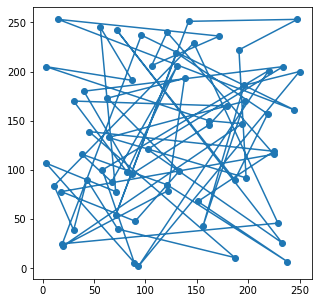
\includegraphics[width=7cm]{figure/tsp_bad.png}
        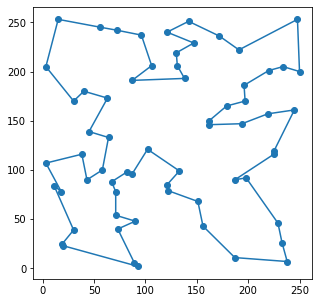
\includegraphics[width=7cm]{figure/tsp_good.png}
        \caption{
            今回の問題設定における巡回セールスマン問題の例\\
            (左) 総距離が大きい経路(総距離: 8437.0)
            (右) 総距離が小さい経路(総距離: 1748.6)
        }
    \end{center}
\end{figure}
\subsection*{巡回セールスマン問題の解法}
巡回セールスマン問題は、NP困難であることが知られている。つまり、厳密な最適解を多項式時間で求めることはできない。
頂点数が20程度の小さな問題であれば、動的計画法によって最適解を求めることができるが、それ以上の規模ではヒューリスティックな手法を用いて最適解に近づける手法が主となる。



